\section{Application Architecture}

\subsection{Overview}

We have decided to build BrainMe using React Native, leveraging the Expo Router for seamless navigation and Convex as our backend solution. Clerk is utilized for robust user authentication. React Native is a popular open-source framework developed by Facebook for building natively compiled applications for multiple platforms using JavaScript and React.

For the development of the application, different services are used, which can be divided into three categories:
\begin{enumerate}
\item \textbf{Device Services:} APIs related to the device's internal functionalities.
\item \textbf{Storage Services:} APIs related to the storage of application data.
\item \textbf{External Services:} APIs related to functionalities and data provided by external companies.
\end{enumerate}

The integration of these services is implemented by using asynchronous communication protocols when possible, ensuring the application remains responsive and smooth regardless of the performance of the external services. \\\\
The internal structure of the app is divided into services, classes, components, and pages following a Model, View, Controller (MVC) pattern. This pattern allows a clear separation between different concepts and makes it easier to replace external services without affecting other parts of the application. \\\\
For device services, React Native libraries help us keep the application device-independent by using wrappers that allow the use of Application Programming Interfaces (API) regardless of the device used. For clarity and to better match the pattern, the same structure is maintained in the source code file structure.

\begin{figure}[H]
\centering
    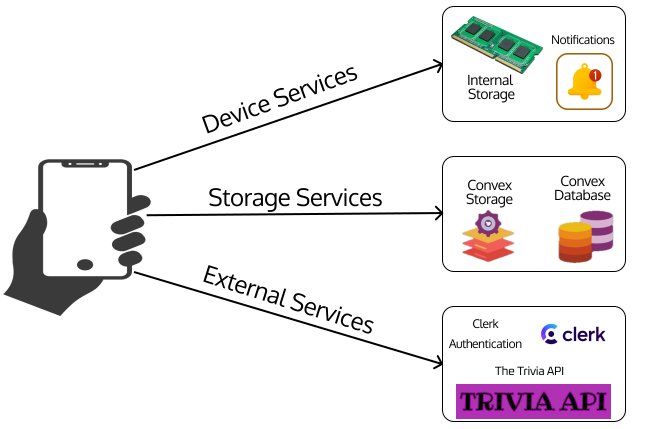
\includegraphics[width=1\textwidth, height=0.4\textheight]{Images/Application Architecture.png}
\caption{Device, Storage, and External Services Integration}
\end{figure}

\subsection{MVC Model: }

The Model represents the data layer of the application, encompassing both the data and the business logic. It is responsible for:

\begin{itemize}

    \item \textbf{Defining Data Structures:} The Model classes structure the data and define the attributes and relationships between different data entities.
    \item \textbf{Business Logic:} The Model contains the logic for data manipulation, validation, and rules enforcement. This ensures that the data remains consistent and accurate.
    \item \textbf{Data Persistence:} The Model interacts with storage services (internal storage and Convex Database) to persist and retrieve data.
\end{itemize}

\subsubsection{The View:}

The View is responsible for presenting the data to the user and handling user interaction. It includes the UI components such as buttons, forms, lists, and displays. The View:

\begin{itemize}

    \item \textbf{Renders the UI:} Displays data from the Model to the user in a readable and interactive format.
    \item \textbf{Receives User Input:} Captures user actions and inputs, such as clicks, typing, and selections.
    \item \textbf{Updates Dynamically:} Reflects changes in the Model by updating the displayed data without reloading the entire page.

\end{itemize}

\subsubsection{The Controller:}

The Controller acts as an intermediary between the Model and the View. It processes user inputs from the View, interacts with the Model to perform actions, and updates the View accordingly. The Controller:

\begin{itemize}

    \item \textbf{Handles User Inputs:} Captures events like button clicks, form submissions, and other user interactions.
    \item \textbf{Manipulates Data:} Calls Model methods to manipulate data based on user actions, ensuring the business logic is executed correctly.
    \item \textbf{Updates the View:} Ensures the View reflects the current state of the Model after data changes or actions.

\end{itemize}

\begin{figure}[H]
\centering
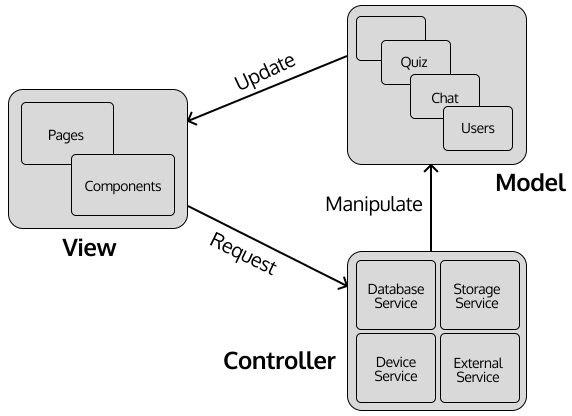
\includegraphics[width=0.8\textwidth]{Images/MVC Pattern.png}
\caption{Model-View-Controller (MVC) Pattern}
\end{figure}

\subsection{Device Services}

Device services in BrainMe include functionalities that are directly related to the device's capabilities:
\begin{enumerate}
\item \textbf{Internal Storage:} Used for storing user data locally on the device, ensuring quick access and offline capabilities.
\item \textbf{Notification:} Handles push notifications to keep users informed about updates, new quizzes, messages, and other relevant events.
\end{enumerate}

\subsection{Storage Services}

Storage services are crucial for data persistence and retrieval:
\begin{enumerate}
\item \textbf{Internal Storage:} Utilized for storing user preferences and other important data locally.
\item \textbf{Convex Database:} Serves as the primary database for storing structured data related to users, quizzes, messages, and leaderboard information.
\end{enumerate}

\subsection{External Services}

External services extend the functionality of BrainMe by integrating third-party APIs:
\begin{enumerate}
\item \textbf{Clerk Authentication:} Manages user authentication processes, including email/password logins and Single Sign-On (SSO) via Google and Apple.
\item \textbf{The Trivia API:} Provides quiz questions categorized by genre and level to enhance the learning experience.
\end{enumerate}

\subsection{Data Model}

Data shown in the application pages has been structured using classes which represent the Model part of the MVC pattern. The following objects are defined to structure the data appropriately:
\begin{enumerate}
\item \textbf{UserModel:} Contains information about registered users, including personal details and preferences.
\item \textbf{QuizModel:} Stores information about quizzes, including genre, level, and associated questions provided by The Trivia API.
\item \textbf{LeaderboardModel:} Tracks user performance and rankings within the application.
\item \textbf{MessageModel:} Contains attributes for messages sent and received within the app’s chat functionality.
\item \textbf{StatisticsModel:} Contains the detailed statistics such as points, correct answers ration, level, games played and so on.
\item \textbf{ChatModel:} Contains the detailed information about the users interacting with each other such as name, chats and the time stamp of when the message was sent and received.

\end{enumerate}

Data is fetched from different sources and is parsed using utility functions to obtain the desired structure. This ensures that the data presented in the application is accurate and up-to-date.